% Vorlage für eine Bachelorarbeit
% Siehe auch LaTeX-Kurs von Mathematik-Online
% www.mathematik-online.org/kurse
% Anpassungen für die Fakultät für Mathematik
% am KIT durch Klaus Spitzmüller und Roland Schnaubelt Dezember 2011

\documentclass[12pt,a4paper]{scrartcl}
% scrartcl ist eine abgeleitete Artikel-Klasse im Koma-Skript
% zur Kontrolle des Umbruchs Klassenoption draft verwenden


% die folgenden Packete erlauben den Gebrauch von Umlauten und ß
% in der Latex Datei
\usepackage[utf8]{inputenc}
% \usepackage[latin1]{inputenc} %  Alternativ unter Windows
\usepackage[T1]{fontenc}
\usepackage[ngerman]{babel}


\usepackage[pdftex]{graphicx}
\usepackage{latexsym}
\usepackage{amsmath,amssymb,amsthm}
\usepackage{setspace}
\usepackage{url}
\usepackage{mathtools}
\usepackage{enumitem}


% Abstand obere Blattkante zur Kopfzeile ist 2.54cm - 15mm
\setlength{\topmargin}{-15mm}


% Umgebungen für Definitionen, Sätze, usw.
% Es werden Sätze, Definitionen etc innerhalb einer Section mit
% 1.1, 1.2 etc durchnummeriert, ebenso die Gleichungen mit (1.1), (1.2) ..
\theoremstyle{definition}
\newtheorem{Satz}{Satz}[section]
\newtheorem{Definition}[Satz]{Definition} 
\newtheorem{Lemma}[Satz]{Lemma}		   
                  
\numberwithin{equation}{section} 

\newtheorem*{Bemerkung}{Bemerkung}

% einige Abkuerzungen
\newcommand{\C}{\mathbb{C}} % komplexe
\newcommand{\K}{\mathbb{K}} % komplexe
\newcommand{\R}{\mathbb{R}} % reelle
\newcommand{\Q}{\mathbb{Q}} % rationale
\newcommand{\Z}{\mathbb{Z}} % ganze
\newcommand{\N}{\mathbb{N}} % natuerliche

% eigene Definitionen
\newcommand{\dx}{\, \mathrm{d} x}
\newcommand{\da}{\, \mathrm{d} a}
\newcommand{\icol}[1]{%inline row vector
		\left(	\begin{smallmatrix}#1\end{smallmatrix} \right) %
	}
\newcommand{\abs}[1]{| #1 |}
\newcommand{\ubar}[1]{\underline{#1}{}}
\DeclareMathOperator{\dive}{div}
\DeclareMathOperator{\spann}{span}
\DeclareMathOperator{\conv}{conv}

\begin{document}
  % Keine Seitenzahlen im Vorspann
  \pagestyle{empty}
  
  
  % Titelblatt der Arbeit
  \begin{titlepage}

    
\includegraphics[scale=0.45]{kit-logo.jpg} 
    \vspace*{2cm} 

 \begin{center} \large 
    
    Bachelorarbeit
    \vspace*{2cm}

    {\huge Die Multilevel Monte Carlo Methode und deren Anwendung am Beispiel der linearen Transportgleichung}
    \vspace*{2.5cm}

    Tim Buchholz
    \vspace*{1.5cm}

    ??.??.??
    \vspace*{4.5cm}


    Betreuung: Prof.Dr. Christian Wieners und M.Sc. Niklas Baumgarten \\[1cm]
    Fakultät für Mathematik \\[1cm]
		Karlsruher Institut für Technologie
  \end{center}
\end{titlepage}



  % Inhaltsverzeichnis
  \tableofcontents

\newpage
 


  % Ab sofort Seitenzahlen in der Kopfzeile anzeigen
  \pagestyle{headings}

\section{Einleitung}
% !TeX root = bachelorarbeit.tex

\section{Einleitung}

Monte Carlo Methoden sind weit verbreitet, um in unterschiedlichsten Situationen Erwartungswerte stochastischer Modelle zu schätzen.
So werden bei der Monte Carlo Quadratur, der wohl bekanntesten Anwendungen der Monte Carlo Methode, zufällig gleichverteilte Stützstellen dafür genutzt, den Erwartungswert der Funktionsauswertung an einer zufälligen Stützstelle zu bestimmen. Daraus lässt sich anschließend der approximierte Integralwert auf einer gegebenen Grundmenge bestimmen. 
Wir wollen Monte Carlo Methoden dazu nutzen, eine stochastische partielle Differentialgleichung zu lösen. 
Genauer betrachten wir eine stochastisch beeinflusste Zielgröße $ Q $ der Lösung der Differentialgleichung und fragen uns, welchen Wert $ \mathbb{E}[Q] $ nimmt $ Q $ im Mittel an? Wir suchen also nach einem Erwartungswert, was die Verwendung von Monte Carlo Methoden zumindest einmal nahelegt. 
Außerdem wollen wir uns dabei die Vorteile der sogenannten Multilevel Monte Carlo (MLMC) Methode zunutze machen. Diese wurde zunächst von Heinrich für Approximation von parameterabhängigen Integralen in hohen Dimensionen entwickelt (vgl. \cite{heinrich2001multilevel}) und anschließend unter anderem von  Giles auf stochastisch modellierte partielle Differentialgleichungen übertragen. Folgendes Zitat bringt die Vorteile auf den Punkt, welche die Multilevel Monte Carlo Methode in diesem Zusammenhang bietet:
\begin{quote}
	\textit{Monte Carlo methods are a very general and useful approach for the estimation of expectations arising from stochastic simulation. However, they can be computationally expensive, particularly when the cost of generating individual stochastic samples is very high, as in the case of stochastic PDEs. \\ Multilevel Monte Carlo is a recently developed approach which greatly reduces the computational cost by performing most simulations with low accuracy at a correspondingly low cost, with relatively few simulations being performed at high accuracy and a high cost.}  \\
	\rightline{Michael B. Giles in \cite{giles_2015}. \, \qquad \qquad }
\end{quote}
Das Lösen, bzw. in unserem Fall das Bestimmen eines Erwartungswert, von stochastisch modellierten partiellen Differentialgleichungen fallen in das Gebiet der Uncertainty Quantification. Dieses noch recht 'junge' Feld der Mathematik wird von Sullivan in \cite{sullivan2015introduction} als ein 'Zusammentreffen der Wahrscheinlichkeitstheorie, Numerik, Statistik und der echten Welt' beschrieben. \\
Die Thesis lässt sich aktuellen Arbeiten am Institut für Angewandte und Numerische Mathematik, wie etwa \cite{BAUMGARTEN2020}, zuordnen und soll daher zwar zum einen den theoretischen Hintergrund darlegen, aber auch einige Ergebnisse präsentieren, die im parallelen Finite Elemente System M++ \cite{siteM++} erzielt werden konnten, welches am Institut für Angewandte und Numerische Mathematik unter anderem von Herrn Prof. Dr. C. Wieners entwickelt wurde. \\
Konkret wollen wir vor allem die zeitabhängige lineare Transportgleichung betrachten. Dabei handelt es sich um ein weit verbreitetes Modellproblem, welches unter Anderem auch in \cite{di2011mathematical}, einem Standardwerk für Discontinuous Galerkin Methoden, zu finden ist. 
Dabei nutzen wir wie in \cite{di2011mathematical} die sogenannte 'method of lines': Zur numerischen Lösung der Differentialgleichung nutzen wir ein Discontinuous Galerkin Verfahren (DGV) im Ort und kombinieren diese zunächst semidiskrete Lösung mit einem geeigneten Zeitschrittverfahren. Aufgrund der Wahl eines Runge-Kutta Verfahrens erhalten wir somit ein Runge-Kutta Discontinuos Galerkin Verfahren. Einen Überblick über diese Verfahrensart findet man zum Beispiel auch in \cite{cockburn2001runge}.
Ebenfalls mit der Anwendung von Multilevel Monte Carlo Methoden auf eine Variante des Transportproblems mit Diffusion haben sich zum Beispiel auch Barth und Stein in \cite{barth2013multilevel} bzw. \cite{barth2019multilevel} oder Kumar et al. in \cite{kumar2018multigrid} beschäftigt. Mit Multilevel Monte Carlo Methoden im Allgemeinen haben sich neben den bereits erwähnten Giles und Barth auch Cliffe in \cite{cliffe2011multilevel}, Charrier in \cite{charrier2012strong} oder Teckentrup in \cite{teckentrup2013further}, um nur Einige zu nennen, befasst.
Um die eigentliche Idee der Multilevel Monte Carlo Methode in den Vordergrund zu rücken, wollen wir diese aber auch wie in \cite{heinrich2001multilevel} am Beispiel der numerischen Integration betrachten.
Dabei wollen wir insbesondere die Unterschiede zu und Vorteile gegenüber der Standard Monte Carlo Methode hervorheben, welche im Kern bereits durch obiges Zitat zusammengefasst sind.

%Monte Carlo Methoden sind weit verbreitet und finden in verschiedenen Bereichen der Mathematik ihre Anwendung.
%Sie dienen dabei als statistische Schätzer für Erwartungswerte. 
%Eine der bekanntesten Anwendungen ist wohl die Monte Carlo Quadratur, welche zur numerischen Integration genutzt werden kann.
% 
%Nachdem Giles (cite ...) ... gewöhnliche DGL ... kam ... für SPDE's zu nutzen ...cite .
%
%
%Allerdings besitzt die Monte Carlo Methode einen entscheidenden Nachteil, will man sie im Zusammenhang unsicherer Ausgangsdaten für die Lösung von partiellen Differentialgleichungen nutzen, sie konvergiert im Normalfall relativ langsam und das numerische Lösen von PDE's ist oft sehr aufwendig.
%Es werden also unter Umständen sehr viele, sehr teure Zufallssamples benötigt, um ein vernünftiges Ergebnis zu erhalten. \newline
%Diese Thesis soll sich daher mit der Multilevel Monte Carlo Methode (im Folgenden MLMC Methode genannt) beschäftigen, welche an die Monte Carlo Methode angelehnt ist, aber durch die geschickte Auswertung der (Zufalls-Samples) deutliche Effizienzvorteile gegenüber der Standard Monte Carlo Methode besitzt.
%Die MLMC Methode soll nach einer ausführlichen theoretischen Analyse auch praktisch auf das Transportproblem angewandt werden.
%Genauer soll für
%\begin{itemize}
%	\item ein beschränktes Gebiet $\mathbb{D} \subseteq \R^d$
%	\item  ein Zeitintervall $\mathbb{T} = [0,T]$
%	\item  ein Wahrscheinlichkeitsraum $(\Omega,\mathcal{A},\mathbb{P})$
%	\item  ein zufälliges Flussvektorfeld $q: \Omega \times \overline{\mathbb{D}} \rightarrow \R^d$
%	\item  eine Anfangskonzentration eines (zu transportierenden) Stoffes $\rho_0: \overline{\mathbb{D}} \rightarrow \R^d$
%	\item einen Einfluss $\rho_{\text{in}} : \Gamma_{\text{in}} \times \mathbb{T} \rightarrow \R$ über den Einflussrand $\Gamma_{\text{in}} \coloneqq  \{ z \in \partial \mathbb{D}: q(z)\cdot n(z) \leq 0 \} \subset  \partial \mathbb{D}$ mit $n(z)$ als äußeren Normalenvektor im (Rand-)Punkt $z$
%\end{itemize}
%der Erwartungswert eines Funktionals der  Konzentration des Stoffes $\rho: \overline{\mathbb{D}} \times \mathbb{T}  \rightarrow \R_{\geq0}$ bestimmt werden. Dabei erhält man $\rho$ als Lösung der folgenden partiellen Differentialgleichung:
%\begin{gather*}
%\text{Bestimme } \rho: \overline{\mathbb{D}} \times \mathbb{T} \to \R_{\geq 0} \text{, sodass}\\
%(\text{TP})
%\begin{cases}
%\partial_t \rho + \dive(\rho q) = 0 &\text{ in } \mathbb{D} \times (0,T)\\
%\rho(x,t) = \rho_{\text{in}}(x,t) &\text{ auf } \Gamma_{\text{in}} \times (0,T)\\
%\rho(x,0) = \rho_0(x) &\text{ auf } \mathbb{D}.
%\end{cases}
%\end{gather*}
%Außerdem muss zunächst ein zwar zufälliges, aber dennoch sinnvolles Vektorfeld $q$ erzeugt werden. Wir nutzen hierbei das Darcy-Gesetz, welches als Modellierung von Fluiden in porösen Bodenschichten bereits oft genutzt wurde (vgl. z.B. \cite{de1986quantitative}).
%Dabei soll später, bevor wir das eigentliche Transportproblem lösen, stets zunächst für einen zufälligen Permeabilitätstensor, welcher die unbekannte Bodenbeschaffenheit modellieren soll, ein entsprechendes Flussvektorfeld $q$ über das sogenannte Potentialströmungsproblem, welches sich aus dem Darcy-Gesetz ableitet, berechnet werden. 
%Die genauere Modellierung des so entstehenden Gesamtproblems soll aber an späterer Stelle erfolgen. \newline
Die Thesis ist dazu folgendermaßen unterteilt:\newline 
Abschnitt 2 sammelt verschiedene Grundlagen aus den Bereichen der Stochastik, der Analysis und der Numerik partieller Differentialgleichungen. Besonders werden wir hierbei auf einige zentrale Aussagen der Wahrscheinlichkeitstheorie eingehen, welche für die Konvergenzanalyse von Monte Carlo Methoden im Allgemeinen eine wichtige Rolle spielen. \newline
In Abschnitt 3 betrachten wir einige Aspekte der (standard) Monte Carlo Methode, welche auch der MLMC Methode als theoretischer Unterbau dienen sollen. Dabei erklären wir die Monte Carlo Methoden zunächst anhand des Beispiels der numerischen Integration, gehen dann aber auch abstrakter auf Konvergenz und Genauigkeit der Methode ein.\newline
Anschließend werden wir in Abschnitt 4 die Multilevel Monte Carlo Methode an sich erklären.
Dazu greifen wir das Beispiel der numerischen Integration aus Abschnitt 3 in einer etwas abgewandelten Form wieder auf. Auch hier wollen wir dann aber etwas abstrakter Eigenschaften der Methode betrachten, welche uns auch später bei der Anwendung auf das Transportproblem wieder beschäftigen werden. \newline
In Abschnitt 5 werden wir dann das Transportproblem einführen und dabei auch das Potentialströmungsproblem beschreiben, welches wir lösen müssen, um an die entsprechenden Ausgangsdaten zu kommen. Anschließend wird die numerische Lösung der beiden Probleme mit Finite Elemente Methoden behandelt, bevor schließlich in Abschnitt 6 auf die Anwendung der Multilevel Monte Carlo Methode auf das Transportproblem mit unsicheren Ausgangsdaten am Beispiel der Permeabilität $\kappa$ eingegangen wird. 
Der siebte und letzte Abschnitt befasst sich mit den konkreten Ergebnissen der Durchführung und Implementierung des zuvor theoretisch beleuchteten Problems innerhalb der parallelen Finite Elemente Softwarebibliothek 'M++' \cite{siteM++}. Außerdem wird auf einige zusätzliche neue Features eingegangen, welche während des praktischen Teils der Thesis erarbeitet wurden. So wurde unter anderem Tools zum Lesen, Verarbeiten und Darstellung von '.vtk'-Dateien, welche in von M++ als Speicherformat genutzt werden, in der Programmiersprache Python implementiert. Neben dem automatisierten Erstellen von Schaubildern auf Grundlage dieser '.vtk'-Dateien, ist es uns außerdem damit möglich, auf Grundlage des durchgeführten Experiments auch eine konkrete MLMC-Lösung zu berechnen. Diese kombiniert die Lösungen, in unserem Fall die Konzentrations\-verläufe, der einzelnen Differentialgleichungen auf die gleiche Weise, wie die Erwartungswerte innerhalb der MLMC Methode verrechnet wurden. Wir erhalten so letztendlich nicht nur den gesuchten Erwartungswert, sondern auch eine auf die Berechnung dieses Erwartungswertes zugeschnittene erwartete Lösung der stochastischen Differentialgleichung. 
Der Thesis ist außerdem ein entsprechendes Notebook beigefügt, mit welchem die Ergebnisse reproduziert werden können.

%%%%%%%%%%%%%%%%%%%%%%%%%%%%%%%%%
 \newpage  % neuer Abschnitt auf neue Seite, kann auch entfallen
%%%%%%%%%%%%%%%%%%%%%%%%%%%%%%%%%
 
\section{Grundlagen}
\subsection{analytische/numerische Grundlagen}
% !TeX root = bachelorarbeit.tex
Sei $\mathcal{D} \subseteq \R^d$ offen für $d\in \N$ und $\lVert \cdot \rVert$ eine Norm auf $\R^d$.
Die folgenden Definitionen und Sätze sollen als Grundlagen für die weiteren Betrachtungen dieser Thesis dienen. Insbesondere wollen wir hierbei meist auf konkrete Beweise verzichten und verweisen dahingehend auf die Literatur. 
Die analytischen Grundlagen bauen zum Teil auf der Vorlesung Rand- und Eigenwertprobleme aus dem Sommersemester 2019 von Herrn Prof. Dr. Reichel auf, sind aber auch  z.B. in \cite{dobrowolski2010angewandte} oder \cite{evans10} zu finden.
\begin{Definition}(Einige Operatoren)
	\begin{enumerate}[label=(\alph*)]
		\item Für $F: \R^d \to \R^d$ ist die \underline{Divergenz} von F definiert durch
			\begin{align*}
				\dive F = \nabla \cdot F \coloneqq \sum_{i=1}^{d} \frac{\partial F_i}{ \partial x_i}
			\end{align*}
		\item Für $f: \R^d \to \R$ und $\alpha = (\alpha_1,\dots,\alpha_d) \in \N^d$ ist die partielle Ableitung von $f$ nach dem sogenannten Multiindex $\alpha$ definiert durch
			\begin{align*}
				\partial^{\alpha}f \coloneqq 
				\frac{\partial^{|\alpha|} f}{\partial x_1 ^{\alpha_1} \cdots  \partial x_d^{\alpha_d} } 
				=\frac{\partial^{\alpha_1+\dots +\alpha_d} f}{\partial x_1 ^{\alpha_1} \cdots  \partial x_d^{\alpha_d} } 
			\end{align*}
	\end{enumerate}
\end{Definition}

%\begin{Satz}
%	Sei $ \mathcal{D} \subset \R^d $ offen und beschränkt und $ 1 \leq p < \infty $, dann gilt: \\
%	$ C_c^{\infty} (\mathcal{D})$ liegt dicht in $ L^p(\mathcal{D}) $, d.h. $ C_c^{\infty}(\mathcal{D}) \subseteq L^p(\mathcal{D})$ und $ \overline{ C_c^{\infty}(\mathcal{D}) }^{\lVert \cdot \rVert_p}  = L^p(\mathcal{D})$
%\end{Satz}


%\begin{Definition}(Lipschitz-Gebiet TODO cite rwp) \newline 
%	\begin{enumerate}[label=(\alph*)]
%		\item Eine offene zusammenhängenden Menge $\mathcal{D} \subset \R^d$ heißt Lipschitz-Gebiet, falls für jedes $x_0 \in \partial \mathcal{D}$ ein Radius $r>0$ und eine Lipschitz-stetige Funktion $\phi : \R^{d-1} \to \R$ existiert, so dass (nach einer geeigneten Bewegung des Koordinatensystems) gilt: \\
%		Für $ x' = (x_1,\dots,x_{d-1})  \text{ und } B_r(x_0) \coloneqq \{ x\in \R^d : \lVert x-x_0 \rVert < r\}  \text{ ist }$
%			\begin{align*}
%				\mathcal{D} \cap B_r(x_0) = \{x = (x',x_d) \in B_r(x_0): x_d > \phi(x')\} 
%			\end{align*}
%		Es gilt dann notwendigerweise:
%			\begin{align*}
%				\partial \mathcal{D} \cap B_r(x_0) = \{x = (x',x_d) \in B_r(x_0): x_d = \phi(x')\}
%			\end{align*}
%		\item Ist $\mathcal{D}$ ein Lipschitz-Gebiet so existiert $x = (x',\phi(x')) \in \partial \mathcal{D} \cap B_r(x_0)$ der Vektor
%			\begin{align*}
%				n(x) = \frac{1}{\sqrt{1+|\nabla \phi(x')|^2}} \icol{\nabla \phi(x')\\-1}
%			\end{align*}
%		fast überall bezüglich des Oberflächenmaßes auf $\partial \mathcal{D}$ und heißt der äußere 
%		Einheitsnormalenvektor an $\partial \mathcal{D}$ im Punkt $x$. 
%	\end{enumerate}
%	
%\end{Definition}


\begin{Satz} (Gaußscher Integralsatz für Lipschitz-Gebiete) \newline
 	Sei $\mathcal{D}  \subset \R^d$ ein beschränktes Lipschitz-Gebiet und sei $n$ der äußere Einheitsnormalenvektor an $\partial \mathcal{D}$. Dann gilt:
 		\begin{align*}
	 		\int_{\mathcal{D}} \frac{\partial f}{\partial x_i} \dx  = \int_{\partial \mathcal{D}} f n_i \da
 		\end{align*}
 		für jede Funktion $f \in C^1(\overline{\mathcal{D}})$. \\ 
 		Oft erscheint der Gaußsche Integralsatz auch in folgender Form:
 		\begin{align*}
 		\int_{\mathcal{D}} \dive F \dx =  \int_{\partial \mathcal{D}} F \cdot n \da
 		\end{align*}
 		wobei $F:\mathcal{D} \to \R^d$ ein Vektorfeld ist. Die Komponentenfunktionen von $F = (F_1,\dots,F_d)$ sollen dann $F_i \in C^1(\overline{\mathcal{D}})$ für $i=1,\dots,n$ erfüllen.
\end{Satz}

\begin{Folgerung}(mehrdimensionale partielle Integration) \\
	\label{n_pI}
	Sei $ u \in C^1(\R^d, \R)$ und $ \vec v : \mathcal{D} \to \R^d $ ein stetig partiell differenzierbares Vektorfeld.
	Dann gilt:
	
	\begin{align*}
		\int_{\mathcal{D}} u \dive ( \vec v) \dx = \int_{\partial \mathcal{D}} u \vec v \cdot n \da
		- \int_{\mathcal{D}} \vec v \cdot \nabla \phi \dx
	\end{align*}
\end{Folgerung}


%\begin{Definition}($ L^1_{\text{loc}} $)\\
%	Todo
%\end{Definition}



\begin{Definition}(schwache Ableitung)\\
	Sei $u \in L_{\text{loc}}^1(\mathcal{D})$. Dabei bezeichne $  L_{\text{loc}}^1(\mathcal{D}) $ den Raum der lokal integrierbaren Funktionen auf $ \mathcal{D} $. Wir sagen v besitzt eine schwache Ableitung zum Multiindex $\alpha$, falls eine Funktion $v \in L_{\text{loc}}^1$ existiert, mit 
		\begin{align*}
			\int_{\mathcal{D}} u \partial^{\alpha} \Phi \dx = (-1)^{|\alpha|} \int_{\mathcal{D}} v \Phi \dx \qquad \forall \Phi \in C_0^{\infty}(\mathcal{D})
		\end{align*}
	In diesem Zusammenhang nennen wir $\Phi$ auch Testfunktion und wir definieren $D^{\alpha} u \coloneqq v$ als die schwache Ableitung von $u$ zum Multiindex $\alpha$. 
\end{Definition}
\begin{Bemerkung}
	Per Konvention ist für $ \alpha = (0,\dots, 0) \quad \partial^{\alpha}u = u $
\end{Bemerkung}
\begin{Definition}(Sobolevräume)\\
	Sei $\mathcal{D} \subseteq \R^d $ offen, $ k \in \N $ und $ 1 \leq p \leq \infty $.  Weiter sei $ L : C^1(\mathcal{D},\R^m) \to L^{\infty}(\mathcal{D},\R^k) $ ein linearer Differentialoperator erster Ordnung und $ L^{\star} : C^1(\mathcal{D},\R^k) \to L^{\infty}(\mathcal{D},\R^m) $ der zugehörige adjungierte Operator. Es gelte also
	\[
	\int_{\mathcal{D}} Lu \cdot \phi \dx = \int_{\mathcal{D}} u \cdot L^{\star} \phi \dx \text{ für } u \in C^1_c(\mathcal{D},\R^m) \text{ , } \phi \in C^1_c (\mathcal{D},\R^k)
	\]
	Dann sind:
	\begin{enumerate}[label=(\alph*)]
		\item $ W^{k,p} (\mathcal{D}) \coloneqq \{ u \in L^p(\mathcal{D})$ und die schwachen Ableitungen $ \partial^{\alpha}u $ existieren, mit $ \partial^{\alpha}u \in L^p(\mathcal{D}) $ für alle $ \alpha \in \N_0^d , |\alpha| \leq k \} $	
		\item $ \lVert u \rVert_{k,p} =  \lVert u \rVert_{W^{k,p}(\mathcal{D})} \coloneqq 
				\begin{cases}
					\begin{array}{lll}
						(\sum\limits_{|\alpha|\leq k} \int_{\mathcal{D}} |\partial^{\alpha} u |^p \dx)^{\frac{1}{p}} &, 1 \leq p < \infty \\
						\sum\limits_{|\alpha|\leq k}   \lVert \partial^{\alpha} u \rVert_{\infty}        &, p = \infty
					\end{array}
				\end{cases}  $
		\item $ W_0^{k,p}(\mathcal{D}) \coloneqq \overline{ C_c^{\infty}(\mathcal{D}) }^{\lVert \cdot \rVert_{k,p}} $. Über den sogenannten Spursatz erhält man eine äquivalente Charakterisierung durch: 
		$ W_0^{k,p}(\mathcal{D}) = \{ v \in W^{k,p}(\mathcal{D}) : v|_{\partial \mathcal{D}} = 0 \}$
		\item Im Falle $ p = 2 $ schreibt man aufgrund der Tatsache, dass es sich dann bei $ W^{k,p}(\mathcal{D}) $ um einen Hilbertraum handelt, oft auch $ H^k(\mathcal{D}) \coloneqq W^{k,p}(\mathcal{D}) $
		\item $ H(L,\mathcal{D}) \coloneqq \{ u \in L^2(\mathcal{D},\R^m) : \exists v \in L^2(\mathbb{D},R^k) \text{ mit } \int_{\mathcal{D}} v \cdot \phi \dx = \int_{\mathcal{D}} u \cdot L^{\star}\phi \dx \ \forall \phi \in C^1_c(\mathcal{D},\R^k) \}$
	\end{enumerate}
\end{Definition}

\begin{Satz}(Multiplikation mit Testfunktionen und Integration) \\ 
	\label{testfunktionen}
	Sei $\mathcal{D} \subset \R^d$ offen und $u \in L_{\text{loc}}^1(\mathcal{D})$ und $\int_{\mathcal{D}} u \psi \dx = 0 \; \forall \psi \in C_c^{\infty}(\mathcal{D})$ ,\\
	dann gilt $ u \equiv 0 $.
\end{Satz}
%\begin{Satz} (Rechnen mit Differentialoperatoren)
%	todo FEM
%\end{Satz}
%\begin{Definition}
%	Hdiv? todo
%\end{Definition}
\subsection{stochastische Grundlagen}
\subsection{Monte Carlo Methoden}
%%%%%%%%%%%%%%%%%%%%%%%%%%%%%%%%%
\newpage  % neuer Abschnitt auf neue Seite, kann auch entfallen
%%%%%%%%%%%%%%%%%%%%%%%%%%%%%%%%%
\section{Multilevel Monte Carlo Methode (MLMC)}
%%%%%%%%%%%%%%%%%%%%%%%%%%%%%%%%%
\newpage  % neuer Abschnitt auf neue Seite, kann auch entfallen
%%%%%%%%%%%%%%%%%%%%%%%%%%%%%%%%%
\section{MLMC angewandt auf das Transportproblem}
\subsection{Problemstellung}
 % !TeX root = bachelorarbeit.tex
\subsubsection{Deterministisches Problem}
\label{det_prob}
Sei $\mathbb{T} = [0,T]$ ein Zeitintervall für $T>0$ und $\mathcal{D} \subset \R^d , d \in \N$ ein beschränktes, offenes und konvexes Lipschitz-Gebiet mit Rand $ \partial \mathcal{D} = \Gamma_{\text{D}}  \dot{\cup} \Gamma_{\text{N}} $. 
Wie bereits in der Einleitung beschrieben, wollen wir den Transport eines Stoffes in einer porösen Bodenschicht auf Grundlage eines vorhandenen Flusses beschreiben. 
Als modellhaftes Problem soll uns hierfür die Versickerung eines Stoffes unter Hinzunahme der Regenwasserversickerung dienen: In einer porösen Bodenschicht befindet sich zum Zeitpunkt $t=0$ ein Stoff (beispielsweise Öl) in einer gegebenen Anfangskonzentration und -verteilung. Nun sickert Regenwasser in diese poröse Bodenschicht ein. Zusätzlich wollen wir weitere Zuflüsse des Fremdstoffes über den Einflussrand $\Gamma_{\text{in}} \subset \partial \mathcal{D}$ zulassen.
Wir sind letztendlich an der Konzentration dieser Substanz an einer Stelle $x \in \overline{\mathcal{D}}$ zu einem Zeitpunkt $t \in \mathbb{T}$ interessiert. \newline
Bevor allerdings die Konzentration als Lösung des Transportproblems bestimmt werden kann, muss zunächst das Flussvektorfeld $q: \overline{\mathcal{D}} \rightarrow \R^d$ berechnet werden. \newline
Sei hierfür $p: D \rightarrow \R$ der hydrostatische Druck, $\kappa: D \rightarrow (\R_{\text{sym}})^{d \times d}$ der Permeabilitätstensor und $G=(0,0,p_0 g_0)^{\top}$. 
Wie bereits in der Einleitung angedeutet, kann der Fluss des Regenwassers durch das Darcy-Gesetz $q=-\kappa(\nabla p + G)$ modelliert werden.
Durch $u(x) := p(x) + p_0 g_0 x_3$ vereinfacht sich das Darcy-Gesetz zu $q=-\kappa \nabla u$.\newline
Nehmen wir die physikalische Annahme hinzu, dass der Fluss $q$ 'quellfrei' sein soll, also an keiner Stelle Masse verschwinden oder erscheinen kann, erhalten wir das Potentialströmungsproblem:
\[ \text{Bestimme } u:\overline{\mathcal{D}} \to \R \text{ und } q: \overline{\mathcal{D}} \to \R^2 \text{ mit } \newline \]
\[\setlength\arraycolsep{1pt}
\text{(PS)}\begin{cases} 
\begin{array}{rll}
\dive q     &= 0                 &\text{ , } \text{in } \mathcal{D}\\
q           &= - \kappa \nabla u &\text{ , } \text{in }\mathcal{D}\\
u           &= u_D               &\text{ , } \text{auf } \Gamma_D \\
-q \cdot \nu  &= g_N               &\text{ , } \text{auf } \Gamma_N 
\end{array}
\end{cases} \\
\]
\begin{Bemerkung}
	Wir wollen aus verschiedenen Gründen direkt die sogenannte gemischte Formulierung des Potentialströmungsproblem nutzen. Näheres dazu findet sich im nächsten Abschnitt.
\end{Bemerkung}
Anschließend suchen wir die Dichteverteilung $\rho: \mathcal{D} \times \mathbb{T} \rightarrow \R_{\geq0} $ einer transportierten Substanz (in unserem Modell das Öl).  \newline
Gegeben sei dazu die Anfangsverteilung $\rho_0: \mathcal{D} \rightarrow \R_{\geq0}$ und der Einfluss der Substanz über die Zeit
$
\rho_{\text{in}} : \Gamma_{\text{in}} \times \mathbb{T} \rightarrow \R_{\geq0} \text{ mit }  \Gamma_{\text{in}} \coloneqq  \{ z \in \partial \mathcal{D}: q(z)\cdot \nu(z) \leq 0 \} \subset  \partial \mathcal{D}
$.
Dabei ist $\nu(z)$ der äußere Normalenvektor im (Rand-)Punkt $z$.
Wir bedienen uns wieder der Physik und fordern die Erfüllung der Bilanzgleichung
\begin{align*}
\forall K \subseteq \mathcal{D} , t\in \mathbb{T} : \frac{d}{dt} \int_K \rho(x,t) \, \mathrm{d}x + \int_{\partial K} \rho(x,t)q(x)\cdot \nu(x) \, \mathrm{d}a = 0.
\end{align*}
Wenden wir für ein zulässiges $K \subseteq \mathcal{D}$ und $\rho,q \in C^1(\mathcal{D})$ den Satz von Gauß an, erhalten wir
\begin{align*}
\int_K \partial_t \rho(x,t) + \dive (\rho q)(x,t) \, \mathrm{d}x = 0
\end{align*}
und können so die lineare Transportgleichung ableiten:
\begin{align*}
\partial_t \rho + \dive (\rho q) = 0 \text{ in } \mathcal{D} \times (0,T]
\end{align*}
Mit den entsprechenden Rand- und Anfangswerten erhalten wir so:

\[ 
\text{Bestimme } \rho: \overline{\mathcal{D}} \times \mathbb{T} \to \R_{\geq 0} \text{, sodass} \newline \]
\[\setlength\arraycolsep{1pt}
\text{(TP)}\begin{cases} 
\begin{array}{rlll}
\partial_t \rho + \dive(\rho q) &= 0 &\text{ , in } &\mathcal{D} \times (0,T)\\
\rho(x,t) &= \rho_{\text{in}}(x,t) &\text{ , auf } &\Gamma_{\text{in}} \times (0,T)\\
\rho(x,0) &= \rho_0(x) &\text{ , auf } &\mathcal{D} \\
\end{array}
\end{cases} \\
\]

\subsubsection{Probabilistisches Problem}
\label{Probabilistisches Problem}
In dem letzten Unterabschnitt sind wir bereits bei der Lösung des Potentialströmungsproblems davon ausgegangen, sämtliche benötigten Randwerte sowie den Permeabilitätstensor $\kappa$ exakt für das gesamte Gebiet $\mathcal{D}$ zu kennen.
Wir wollen uns von dieser durchaus starken Annahme lösen und deshalb zusätzlich die Permeabilität $\kappa$ mit Mitteln der Stochastik modellieren.
Sei dazu $(\Omega, \mathcal{A},\mathbb{P})$ ein Wahrscheinlichkeitsraum und ab nun $d=2$, also $\mathcal{D} \subseteq \R^2$.
\begin{Bemerkung}
	Grundsätzlich funktionieren die vorgestellten Verfahren auch für $d=3$, wir wollen uns aber der Anschaulichkeit halber auf zwei Dimensionen beschränken. Das so betrachtete Gebiet $\mathcal{D}$ lässt sich so z.B. als Querschnitt einer Bodenschicht interpretieren.
\end{Bemerkung} 
Weiter sei nun $\kappa (\cdot,x): \Omega \rightarrow \R_{\geq0}$ die (vom Zufall abhängige) Permeabilität.
Wie schon an anderer Stelle (z.B. in \cite{kumar2018multigrid}) wollen wir die Permeabilität als lognormal-Feld modellieren.
Unser so entstehendes Problem fällt somit in den Bereich der Uncertainty Quantification und ist gegeben durch: 


\begin{align*}
\setlength\arraycolsep{1pt}
&\text{Für jedes benötigte } \omega \in \Omega \text{, bestimme } u(\omega,\cdot):\overline{\mathcal{D}} \to \R \text{ und } q(\omega, \cdot): \overline{\mathcal{D}} \to \R^2 \text{ mit } \\
&\text{(PS)}
	\begin{cases}
		\begin{array}{rlll}
		\dive (q(\omega,x)) &= 0  &\text{, für } x \in \mathbb{ D}\\  
		q(\omega,x) &= - \kappa(\omega) \nabla u(\omega,x)  &\text{, für } x \in \mathcal{D}\\
		-q(\omega,x) \cdot \nu(x) &= g_N(x)  &\text{, für } x \in \Gamma_N \\
		u(\omega,x) &= u_D(x)  &\text{, für } x \in \Gamma_D \\
		\end{array}
	\end{cases} \\
&\text{Für } q: \Omega \times \overline{\mathcal{D}} \to \R^2 \text{, bestimme }\rho: \Omega \times \overline{\mathcal{D}} \times \mathbb{T} \to \R_{\geq 0} \text{ mit} \\
&\text{(TP)} 
	\begin{cases}
		\begin{array}{rlll}
			\partial_t \rho (\omega, x, t) + \dive(\rho(\omega,x,t)q(\omega,x)) &= 0 &\text{, für } (x,t) \in \mathcal{D} \times (0,T] \\
			\rho(\omega,x,t) &= \rho_{\text{in}}(x,t) &\text{, für } (x,t) \in \Gamma_{\text{in}} \times \mathbb{T} \\
			\rho(\omega,x,0)  &= \rho_0(x) &\text{, für } x \in  \mathcal{D}
		\end{array}
	\end{cases} \\
&\text{ für die Anfangs- und Randwerte: } \\ 
	&\begin{array}{llr}
		g_N&: \Gamma_{\text{N}} \to \R \\
		u_D&: \Gamma_{\text{D}} \to \R \\
	    \rho_{\text{in}}&: \Gamma_{\text{in}} \times \mathbb{T} \to \R_{\geq0} \\
		\rho_0&: \mathcal{D} \to \R_{\geq0} \\
	\end{array} \newline \\
&\text{ wobei } \partial \mathcal{D} = \Gamma_{\text{D}} \dot{\cup} \Gamma_{\text{N}}  \text{ und }  \Gamma_{\text{in}} \coloneqq  \{ z \in \partial \mathcal{D}: q(z)\cdot \nu(z) \leq 0 \} \subset  \partial \mathcal{D}
\end{align*}
Dabei stellen wir uns die Aufgabe, den Erwartungswert eines gegebenen Zielfunktionals $Q(\rho(\omega))$ zu berechnen, etwa dem Ausfluss der transportierten Substanz über den Rand. An dieser Stelle können wir dann, nachdem wir uns in den nächsten zwei Unterabschnitten damit beschäftigt haben, wie wir obige Probleme numerisch lösen, die MLMC Methode nutzen, um diesen Erwartungswert zu berechnen. 

\subsection{Numerische Lösung des Potentialströmungsproblem}
% !TeX root = bachelorarbeit.tex
\label{num_pot}
\begin{Bemerkung}
	Die beiden folgenden Abschnitte bauen im Wesentlichen auf den beiden Vorlesungen 'Einführung in das Wissenschaftliche Rechnen' (SS 2019) und 'Finite Elemente Methoden' (WS 2019/2020) von Herrn Prof. Dr. Wieners auf. Dem entsprechend sind als Quellen neben \cite{brenner2007mathematical},
	\cite{braess2013finite} und \cite{hanke2002grundlagen} vor allem die Mitschriebe zu den oben genannten Vorlesungen, sowie die Berichte zum Rechnerpraktikum mit M++ \cite{siteM++} zu nennen.
\end{Bemerkung}
Wie bereits in obigem Abschnitt erwähnt, sollen sich die nächsten beiden Abschnitte damit beschäftigen, wie wir die oben beschriebenen Probleme für ein festes $\omega \in \Omega$ numerisch lösen können. 
Wir wollen dabei im Folgenden auf eine Möglichkeit eingehen, diese Berechnung numerisch durchzuführen. Insbesondere werden dabei jene Verfahren beschrieben, welche wir auch später innerhalb der MLMC Methode in M++ nutzen wollen.
Da wir in diesen beiden Abschnitten $\omega \in \Omega$ ohnehin festhalten, genügt es zudem das deterministische Problem zu betrachten. \newline
Sowohl das hybride Finite Elemente Verfahren, welches wir zur Lösung des Potentialströmungsproblem nutzen wollen, als auch das Discontinuous Galerkin Vefahren, mit dessen Hilfe wir das Transportproblem lösen wollen, bauen auf der Finite Elemente Theorie auf. 
Diese ist im Wesentlichen in der zweiten Hälfte des 20. Jahrhunderts entstanden, ist aber bis heute in praktischer wie auch in theoretischer Sicht aktuell.
Die Grundidee ist hierbei, die vorliegenden Rand-Anfangswertaufgaben in einem passenden endlichen Unterraum zu lösen. Dabei löst man sich auf analytischer Seite zunächst oft von einzelnen Regularitäts- und Differenzierbarkeitsbedingungen und führt einen sogenannten schwachen Lösungsbegriff ein (vergleiche Abschnitt 2.1). Statt nun aber solch eine schwache Lösung in einem unendlich dimensionalen Funktionenraum, wie beispielsweise in den Sobolevräumen $H^1(\mathcal{D})$ oder $H_0^1(\mathcal{D})$ zu bestimmen, zieht man sich auf endlich dimensionale Unterräume zurück. \newline
Die folgende Definition entstammt \cite{brenner2007mathematical} und geht ursprünglich (1978) auf Ciarlet zurück.
\begin{Definition}\
	Sei
	\begin{itemize}
		\item $K \subseteq \R^d$ eine beschränkte abgeschlossene Menge mit einem nichtleeren Inneren und stückweise stetig differenzierbarem Rand 
		\item $\mathcal{P}$ ein endlich dimensionaler Funktionenraum auf K
		\item $\Xi = \{\eta_1,\eta_2,\dots,\eta_k \}$ eine Basis für $\mathcal{P}^{'}$
	\end{itemize}
	Dann heißt $(K,\mathcal{P},\Xi)$ ein finites Element.
\end{Definition}

Wir wollen im Folgenden diese theoretische Definition zwar im Hinterkopf behalten, aber wie in \cite{braess2013finite} meist nur mit den sogenannten Finite-Elemente-Räumen arbeiten. 
Dabei wird eine geeignete Zerlegung $\mathcal{T} = \{K_1,K_2,\dots, K_M \}$ von $\mathcal{D}$ in endlich viele Teilgebiete gewählt. 
Anschließend betrachten wir einen endlichen Raum von Funktionen, die eingeschränkt auf diese Teilgebiete von einfacher Gestalt sind, beispielsweise bieten sich oft polynomielle Darstellungen niedrigen Grades an. 
Ein solches Teilgebiet $K \in \mathcal{T}$ nennen wir Finites Element oder auch Zelle und fordern implizit, verbunden mit dem betrachteten Funktionenraum, die Erfüllung der obigen Definition. \newline
Im Falle $\mathcal{D} \subseteq \R^2$ kommen so z.B. Dreiecke oder Vierecke in Frage, in $\mathcal{D} \subseteq \R^3$ können Tetraeder, Würfel, Quader und andere genutzt werden. \newline
Sei nun $\mathcal{D} \subseteq \R ^2$ zudem ein polygonales Gebiet, um eine einfache Zerlegung in Dreiecke oder Vierecke zu gewährleisten.

\begin{Definition}
	\label{FEMDISC}
	\begin{enumerate}
		\item Eine Zerlegung $\mathcal{T} = \{ K_1,K_2,\dots,K_M\}$ von $\mathcal{D}$ in Dreiecks- oder Viereckselemente heißt zulässig, wenn folgende Eigenschaften erfüllt sind:
		\begin{itemize}
			\item $\overline{\mathcal{D}} = \bigcup_{i=1}^M K_i$
			\item Für $i \neq j$ ist $K_i\cap K_j$
			\begin{enumerate}
				\item ein gemeinsamer Eckpunkt von $K_i$ und $K_j$
				\item eine gemeinsame Kante von $K_i$ als auch von $K_j$
				\item oder $K_i\cap K_j= \emptyset$
			\end{enumerate}
			
		\end{itemize}
		\item Wir schreiben oft $\mathcal{T}_h$ anstatt $\mathcal{T}$, wenn jedes Element einen Durchmesser von höchstens $h$ besitzt .
		\item Eine Familie von Zerlegungen $ \{ \mathcal{T}_h \} $ heißt uniform, wenn ein $ \delta > 0  $ existiert, sodass jedes $ K \in \mathcal{T}_h $ einen Kreis mit Radius $ r_K $ enthält mit $ r_K \geq \frac{h}{\delta} $ .
	\end{enumerate}
\end{Definition}

\begin{figure}[H]
	\centering
	\captionabove{Zulässige Zerlegung und unzulässige Zerlegung mit hängendem Knoten}
	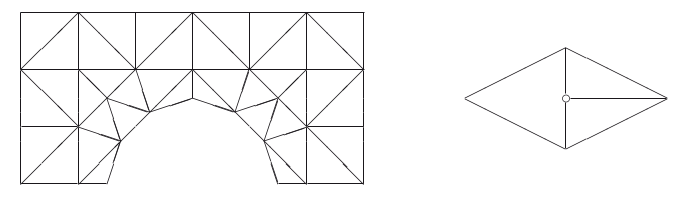
\includegraphics[width=0.8\textwidth]{triangulierung.png} \\
	Abbildung aus \cite{braess2013finite} Seite 58
\end{figure}
Wir werden außerdem im Laufe der Thesis dazu übergehen, ähnlich wie bereits im Abschnitt über die Multilevel Monte Carlo Methode auch bei Zerlegungen von 'Leveln' zu sprechen. Dabei betrachten wir stets eine uniforme Familie zulässiger Zerlegungen $ \{\mathcal{T}_h\}_{h \in \mathcal{H}} $ und fordern dabei, dass die Indexmenge $ \mathcal{H} $ eine ganz bestimmte Form hat. Genauer soll \[ \mathcal{H} = \{ h_0 , h_1 \coloneqq \frac{h_0}{2},h_2 \coloneqq \frac{h_1}{2} = \frac{h_0}{4}, \dots \}  \text{ für ein }  h_0 > 0  \] gelten. Insbesondere gelte also $ \overline{\mathcal{H}} \ni 0 $. Sprechen wir dann von Level $ i $ meinen wir damit die Zerlegung $\mathcal{T}_{h_i} \in \{\mathcal{T}_h\}$.
Zudem führen wir für alle Zerlegungen folgende Bezeichnungen ein:
\begin{itemize}
	\item ein $ K \in \mathcal{T} $ nennen wir Zelle
%	\item $ \mathcal{D}_h \coloneqq \bigcup_{K \in \mathcal{T}} K $ sei die Menge der Zellen
	\item ein $ z \in \mathcal{V}_K \coloneqq \{ z_{K,0} , z_{K,1} , z_{K,2}, z_{K,3}\} \subset \R^2 $ nennen wir Knoten und $\mathcal{V}_K$ die Menge der Knoten von K
	\item $ \mathcal{V}_{\mathcal{T}} \coloneqq \bigcup_{K \in \mathcal{T}} \mathcal{V}_K $ sei die Menge aller Knoten
	\item $\mathcal{F}  \coloneqq (\{ \partial K_1 \cap \partial K_2 : K_1,K_2 \in \mathcal{T} \} \cup \{ \partial K_1 \cap \partial \mathcal{D} : K_1 \in \mathcal{T} \}) \setminus \{\emptyset\} $ sei die Menge aller Seiten
	\item $ \mathcal{F}_K \coloneqq (\{ \partial K \cap \partial K' : K' \in \mathcal{T} \} \cup \{ \partial K \cap \partial \mathcal{D} \}) \setminus \{ \emptyset \} $ sei die Menge aller Seiten von K 
	\item $ \partial \mathcal{D}_h \coloneqq \bigcup_{F \in \mathcal{F}} F $ sei der Rand von $ \mathcal{D}_h $.
\end{itemize}

\subsubsection{Schwache Formulierung}
Betrachten wir also die deterministische Version des Potentialströmungsproblem:
\[ \text{Bestimme } u:\overline{\mathcal{D}} \to \R \text{ und } q: \overline{\mathcal{D}} \to \R^2 \text{ mit } \newline \]
\[\setlength\arraycolsep{1pt}
\text{(PS)}\begin{cases} 
\begin{array}{rlcr}
\dive q     &= 0                 &\text{ ,} \text{in } \mathcal{D} &(1)\\
q           &= - \kappa \nabla u &\text{ ,} \text{in }\mathcal{D} &(2)\\
u           &= u_D               &\text{ ,} \text{auf } \Gamma_D \\
-q \cdot n  &= g_N               &\text{ ,} \text{auf } \Gamma_N 
\end{array}
\end{cases} 
\]
Satz \ref{testfunktionen} sagt uns , dass wir in obiger Formulierung Gleichung (1) mit Testfunktionen $\phi \in H^1(\mathcal{D})$ und Gleichung (2) mit Testfunktionen $\psi \in H^1(\dive,\mathcal{D})$ multiplizieren und anschließend über $\mathcal{D}$ integrieren können und so eine äquivalente schwache Formulierung herleiten:
\begin{align*}
	\int_{\mathcal{D}} \dive(q) \phi \dx &= 0 \text{ für alle Testfunktionen } \phi : \mathcal{D} \to \R \\
	\int_{\mathcal{D}} (q + \kappa \nabla u) \cdot \psi \dx &= 0 \text{ für alle Testfunktionen } \psi : \mathcal{D} \to \R^2
\end{align*}
Da $\kappa$ weiter symmetrisch positiv definit ist, lässt sich letztere Gleichung zu 
\begin{align*}
	&\int_{\mathcal{D}} \kappa^{-1} (q + \kappa \nabla u) \cdot \psi \dx = 0 \\
	\Leftrightarrow \qquad &\int_{\mathcal{D}} \nabla u \cdot \psi \dx = - \int_{\mathcal{D}} (\kappa^{-1}q)\cdot \psi \dx \qquad (\star) 
\end{align*}
umformen. Außerdem wollen wir nun noch die Dirichlet-Randbedingungen $u = u_D \text{ auf } \Gamma_{\text{D}}$ einfließen lassen. Dazu verwenden wir den Satz von Gauß:


\[ \int_{\partial\Omega} (u\psi) \cdot n \da \stackrel{\text{Gauß}}{=} 
 \int_{\Omega} \dive(u\psi) \dx = \int_{\Omega} \nabla u \cdot \psi \dx + \int_{\Omega} u \dive(\psi) \dx \quad (\psi:\Omega \to \R^2) \]
Wählen wir nun unseren Ansatzraum so, dass  für die Funktion $ \psi$ gilt $ \psi \cdot n = 0 \text{ auf } \Gamma_N $. Damit folgt
\begin{align*}
\int_{\Gamma_D} (u_D\psi) \cdot n \da \overset{\psi \cdot n|_{\Gamma_N} = 0}{\underset{u |_{\Gamma_D} = u_D} {=}} \int_{\partial\Omega} (u\psi) \cdot n \da = \underbrace{\int_{\Omega} \nabla u \cdot \psi \dx}_{\stackrel{(\star)}{=}- \int_{\Omega} (\kappa^{-1} q) \cdot \psi \dx } + \int_{\Omega} u \dive(\psi) \dx.
\end{align*}
Die Neumann-Randbedingung $ (\kappa\nabla u) \cdot n = g_N \text{ auf } \Gamma_N $ wird durch die Wahl des Lösungsraumes erfüllt.


Wir erhalten so folgende schwache Formulierung:
\label{sPS}
\begin{align*}
&\text{Bestimme } (q,u) \text{ mit } q\cdot n = -g_N \text{ auf } \Gamma_N \text{ und}\\
&\text{(sPS)}\begin{cases}
\begin{array}{llll}
\int_{\mathcal{D}} \kappa^{-1} q \cdot \psi \dx \, - \mkern-15mu &\int_{\mathcal{D}} u \, \dive(\psi) \dx &= - \int_{\Gamma_D} (u_D \psi) \cdot n \da\\
&\int_{\mathcal{D}} \dive(q) \, \phi \dx &= 0
\end{array}
\end{cases}	\\
&\text{ für alle } (\psi, \phi) \text{ in einem geeigneten Testraum mit } \psi \cdot n = 0 \text{ auf } \Gamma_N 
\end{align*}

\subsubsection{Diskretisierung}
Sei $\mathcal{T}  $ eine zulässige Zerlegung von $ \mathcal{D} $ und alle Bezeichnungen wie oben.
Dabei sei im Weiteren $ N \coloneqq \abs{\mathcal{F}} $ die Anzahl der Seiten und $M = \abs{\mathcal{T}}$ die Anzahl der Zellen.
Wir nummerieren zunächst die Zellen und die Seiten durch:
\begin{align*}
	\mathcal{F} &= \{ F_1,\dots,F_{N}\} \qquad \text{globale Seitennummerierung} \\
	\mathcal{T} &=  \{ K_1,\dots,K_{M}\} \qquad \text{globale Zellennummerierung}
\end{align*}
Als Nächstes soll es nun Ziel sein, eine Lösung der im letzten Abschnitt erklärten schwachen Formulierung in einem endlich dimensionalen Finite Elemente Ansatzraum zu bestimmen. Um aber hierfür genau diese Räume definieren zu können, benötigen wir zuerst sogenannte Basisfunktionen, genauer die Seiten- und die Zellenbasis.\\

 \begin{Definition}(Seiten- und Zellenbasis) 
	\begin{enumerate}[label=(\alph*)]
		\item $ \{ \psi_i \}_{i=1}^{N} $ heißt Seitenbasis und ist definiert durch
			\begin{align*}
					\forall i,j \in \{1, \dots , N \} : \int_{F_j} \psi_i \cdot n^K \da = \pm \delta_{i,j} \text{ und }  \psi_i|_K \in \mathbb{P}_1(K,\R^2) \cap C(\overline{\mathcal{D}}) \ (K \in \mathcal{T}) 
			\end{align*} 
		\item $ \{ \mu_i \}_{i=1}^{M} $ heißt Zellenbasis und ist gegeben durch
			\begin{align*}
				\forall i \in \{1, \dots , M \} : \mu_i \coloneqq  \mathds{1}_{K_i}.
			\end{align*}
	\end{enumerate}
\end{Definition} 

Anschließend können wir mithilfe dieser Basisfunktionen die Testräume bzw. Finite Elemente Räume definieren:
\begin{Definition}(Ansatzräume)
	\begin{enumerate}[label=(\alph*)]
		\item $ W_h \coloneqq \spann \{ \psi_1,\dots,\psi_{N}\}$ (Seitenansatzraum/ Raum für $ \psi $ und $ q_h $)
		\item $ W_h(g) \coloneqq \{ \psi_h \in W_h:  \int_F \psi_h \cdot n \da = \int_F g \da \; \text{ für alle } F \subseteq \Gamma_{\text{N}})  \}$
		\item $ \mathcal{Q}_h \coloneqq \spann \{ \mu_1, \dots, \mu_{M} \} $ (Zellenansatzraum/ Raum für $\phi $ und $ u_h $)
	\end{enumerate}
\end{Definition}

%\begin{Bemerkung}
%	
%	\[	\forall K \in \mathcal{K}:\psi_i|_K \in \mathbb{P}_1(K,\R^2) \text{ und } \mu_m|_K \in \mathbb{P}_0(K,\R) \]
%	Also
%	\begin{align*}	
%	W_h &\subseteq \prod_{K \in \mathcal{K}} \mathbb{P}_1(K,\R^2) &&\text{(Menge der zellenweisen linearen Funktionen) und }\\
%	Q_h &\subseteq \prod_{K \in \mathcal{K}} \mathbb{P}_0(K,\R) &&\text{(Menge der zellenweisen konstanten Funktionen)}. 
%	\end{align*}	
%\end{Bemerkung}

Zusammen mit der schwachen Formulierung \eqref{sPS} erhalten wir so das nun diskretisierte Problem:
\begin{align*}
&\text{Bestimme } (q_h,u_h) \in W_h(-g_N) \times \mathcal{Q}_h \text{ mit}\\
&\begin{cases}
\begin{array}{llll}
\int_{\Omega} \kappa^{-1} q_h \cdot \psi_h \dx \, - \mkern-15mu &\int_{\Omega} u_h \, \dive(\psi_h) \dx &= - \int_{\Gamma_D} (u_D \psi_h) \cdot n \da\\
&\int_{\Omega} \dive(q_h) \, \phi_h \dx &= 0
\end{array}
\end{cases}	\\
&\text{ für alle } (\psi_h, \phi_h) \in W_h(0) \times \mathcal{Q}_h
\end{align*} 




\subsection{Formulierung als LGS}
%Es seien wie bisher Seiten, Seitenbasis, Zellen und Zellenbasis global nummeriert 
%\begin{align*}
%&N \coloneqq \abs{\mathcal{F}} &&\mathcal{F} = \{F_1, \dots , F_{N} \}  \\
%&&&W_h =\{\psi_1, \dots , \psi_N\}\\
%&M \coloneqq \abs{\mathcal{K}} &&\mathcal{K} = \{K_1, \dots , K_{M} \}  \\
%&&&Q_h = \{\mu_1 , \dots , \mu_M  \}.
%\end{align*}

Wir können nun damit beginnen, das so entstandene endlich dimensionale Problem in ein Lineares Gleichungs System umzuformulieren. Dazu definieren wir:
	\begin{align*}
	&\underline{A} \in \R^{N \times N} \text{ mit } \underline{A}[n,k] \coloneqq \int_{\Omega} \kappa^{-1} \psi_n \cdot \psi_k \dx \\
	&\underline{B} \in \R^{M \times N} \text{ mit } \underline{B}[m,k] \coloneqq - \int_{\Omega} \mu_m \dive(\psi_k) \dx \\
	&\underline{b} \in \R^N \text{ mit } \underline{b}[k] \coloneqq - \int_{\Gamma_D} u_D \psi_k \cdot n \da
	\end{align*}
	und (für die Randbedingungen)
	\begin{align*}
	\underline{W}(g) \coloneqq \left\{ \underline{q} \in \R^N : \underline{q}[k] = \int_{F_k} g  \da \ (\text{für } k \text{ mit } F_k \subseteq \Gamma_N) \right\} 
	\end{align*}


Unser zu lösendes Problem lässt sich so mit $ q_h = \sum_{n=1}^{N} \underline{q}[n] \psi_n $ und $ u_h = \sum_{m=1}^{M} \underline{u}[m] \mu_m $ umformen zu 
\begin{align*}
\text{Bestimme} (\underline{q},\underline{u}) \in \underline{W}(-g_N)\times \R^{M} \text{ mit }\\
\begin{cases}
\underline{A} \underline{q} + \underline{B}^T \underline{u} &= \underline{b} \\
\underline{B} \underline{q} &= 0
\end{cases}
\end{align*}
oder anders geschrieben 
\begin{align*}
\text{Bestimme} (\underline{q},\underline{u}) \in \underline{W}(-g_N)\times \R^{M} \text{ mit }\\
\begin{cases}
\begin{pmatrix}
\underline{A} &\underline{B}^T\\
\underline{B} &0
\end{pmatrix}
\begin{pmatrix}
\underline{q} \\
\underline{u} 
\end{pmatrix}
=
\begin{pmatrix}
\underline{b}\\
0
\end{pmatrix}.
\end{cases}
\end{align*}

Wir haben so eine diskrete gemischte Formulierung des Potentialströmungsproblems hergeleitet und können mit dieser aus gegebenen Rand- und Anfangswerten ein Flussvektorfeld $q$ erzeugen, welches der obigen Differentialgleichung genügt.
Es handelt sich hierbei um das gemischte Finite Elemente Verfahren. In M++ selbst lösen wir das Potentialströmungsproblem durch eine Abwandlung dieses Verfahrens. Wir diskretisieren dazu eine äquivalente Formulierung von (sPS) und erhalten so mit dem hybriden Finite Elemente Verfahren die gleichen Ergebnisse, die auch der vorgestellte gemischte Ansatz liefern würde, bei besserer Effizienz und guter Parallelisierbarkeit. Da das Potentialströumgsproblem in dieser Thesis primär dazu genutzt werden soll, das Vektorfeld $q$ zu bestimmen, soll uns aus theoretischer Sicht aber obige Formulierung genügen und wir verweisen hinsichtlich der Lösung mit hybriden gemischten Finiten Elementen, neben einem kleinen, Überblick verschaffendem Abschnitt im Appendix \ref{Referenzzelle&Hyb}, auf die Literatur, wie etwa \cite{brezzi2012mixed} oder  \cite{roberts1991mixed}.












\subsection{Numerische Lösung des Transportproblem}

\subsection{Anwendung der MLMC Methode auf das Transportproblem für unsichere Permeabilität $\kappa$ }
%%%%%%%%%%%%%%%%%%%%%%%%%%%%%%%%%
\newpage  % neuer Abschnitt auf neue Seite, kann auch entfallen
%%%%%%%%%%%%%%%%%%%%%%%%%%%%%%%%%
\section{Beispiel/Experiment}
\subsection{Konkretes Problem}

\subsection{Ergebnisse}
%%%%%%%%%%%%%%%%%%%%%%%%%%%%%%%%%
\newpage  % neuer Abschnitt auf neue Seite, kann auch entfallen
%%%%%%%%%%%%%%%%%%%%%%%%%%%%%%%%%
\section{Ausblick und Fazit}

  % Literaturverzeichnis (beginnt auf einer ungeraden Seite)
  \newpage

%\begin{thebibliography}{Lam00}
 %Bibiographie
  \bibliographystyle{abbrv}
  \bibliography{References}
%\end{thebibliography}
 
      
  % ggf. hier Tabelle mit Symbolen 
  % (kann auch auf das Inhaltsverzeichnis folgen)

\newpage
  
 \thispagestyle{empty}


\vspace*{8cm}


\section*{Erkl\"arung}

Ich  versichere  wahrheitsgem\"a\ss,  die  Arbeit selbstst\"andig verfasst,  alle  benutzten  Hilfsmittel  vollst\"andig  und  genau  angegeben  und  alles kenntlich  gemacht  zu  haben,  was  aus  Arbeiten  anderer  unver\"andert  oder  mit  Ab\"anderungen entnommen  wurde,  sowie die Satzung  des  KIT  zur  Sicherung guter wissenschaftlicher Praxis in der jeweils g\"ultigen Fassung beachtet zu haben.
\\[2ex] 

\noindent
Ort, den Datum\\[5ex]

% Unterschrift (handgeschrieben)



\end{document}

